
\section{Decoding Internal Mobility Patterns}\label{sec:internal_mobility_patterns}


Having developed a measure of skill distance between positions based on job postings and validating it, we explore how 
this can be applied to understand mobility patterns within the firm. The measure quantifies the distance between skills 
and tasks enumerated in job postings and assesses selection chances of candidates for new vacancies. In this section, 
we apply the skill distance metric to study how internal candidates' application behaviors vary based on their 
prospects at the time of application. By capturing predictable variation in selection, this measure enables a more 
nuanced examination of internal transitions and application patterns. The firm can now pose more sophisticated queries 
about internal mobility. For instance, it can now assess for any employee the proportion of new vacancies where their 
skill distance suggests a high probability of selection based on historical patterns. Central to our empirical 
investigation is the average skill distance measure, which assesses an employee's prospects for movement within the firm. 
From an internal applicant's perspective, if many vacancies share skills similar to their current job, their prospects are 
good; if most vacancies are distant, their prospects are weaker. We first develop this average skill similarity measure, 
then proceed to a detailed empirical analysis of application patterns and internal mobility. This analysis opens up new 
possibilities for understanding and supporting workforce development.




\subsection{Average Skill Distance}

To formalize the concept of average skill distance introduced above, we define the following metric:

\begin{equation}
    \overline{d}_{j_c, t} = \frac{1}{|J_t|} \sum_{j_v \in J_t} d(j_c, j_v)
\end{equation}

where $\overline{d}_{j_c, t}$ represents the average distance to job postings at time $t$, $J_t$ is the set of job postings in time window $t$, and $d(j_c, j_v)$ is the distance between the current job $j_c$ and a vacancy $j_v$. In our empirical analysis, we compute this measure for each internal applicant, considering all vacancies in a 30-day window prior to their observed application. This approach allows us to quantify an employee's prospects at the time of application, as discussed in the preceding paragraph. The distribution of $\overline{d}_{j_c, t}$, illustrated in \autoref{fig:s_dist_hist}, reveals notable heterogeneity in applicants' average skill distances, providing a foundation for our subsequent analysis of application patterns and internal mobility.

\begin{figure}[h]
    \begin{center}
        \begin{minipage}{\textwidth}
            \centering
            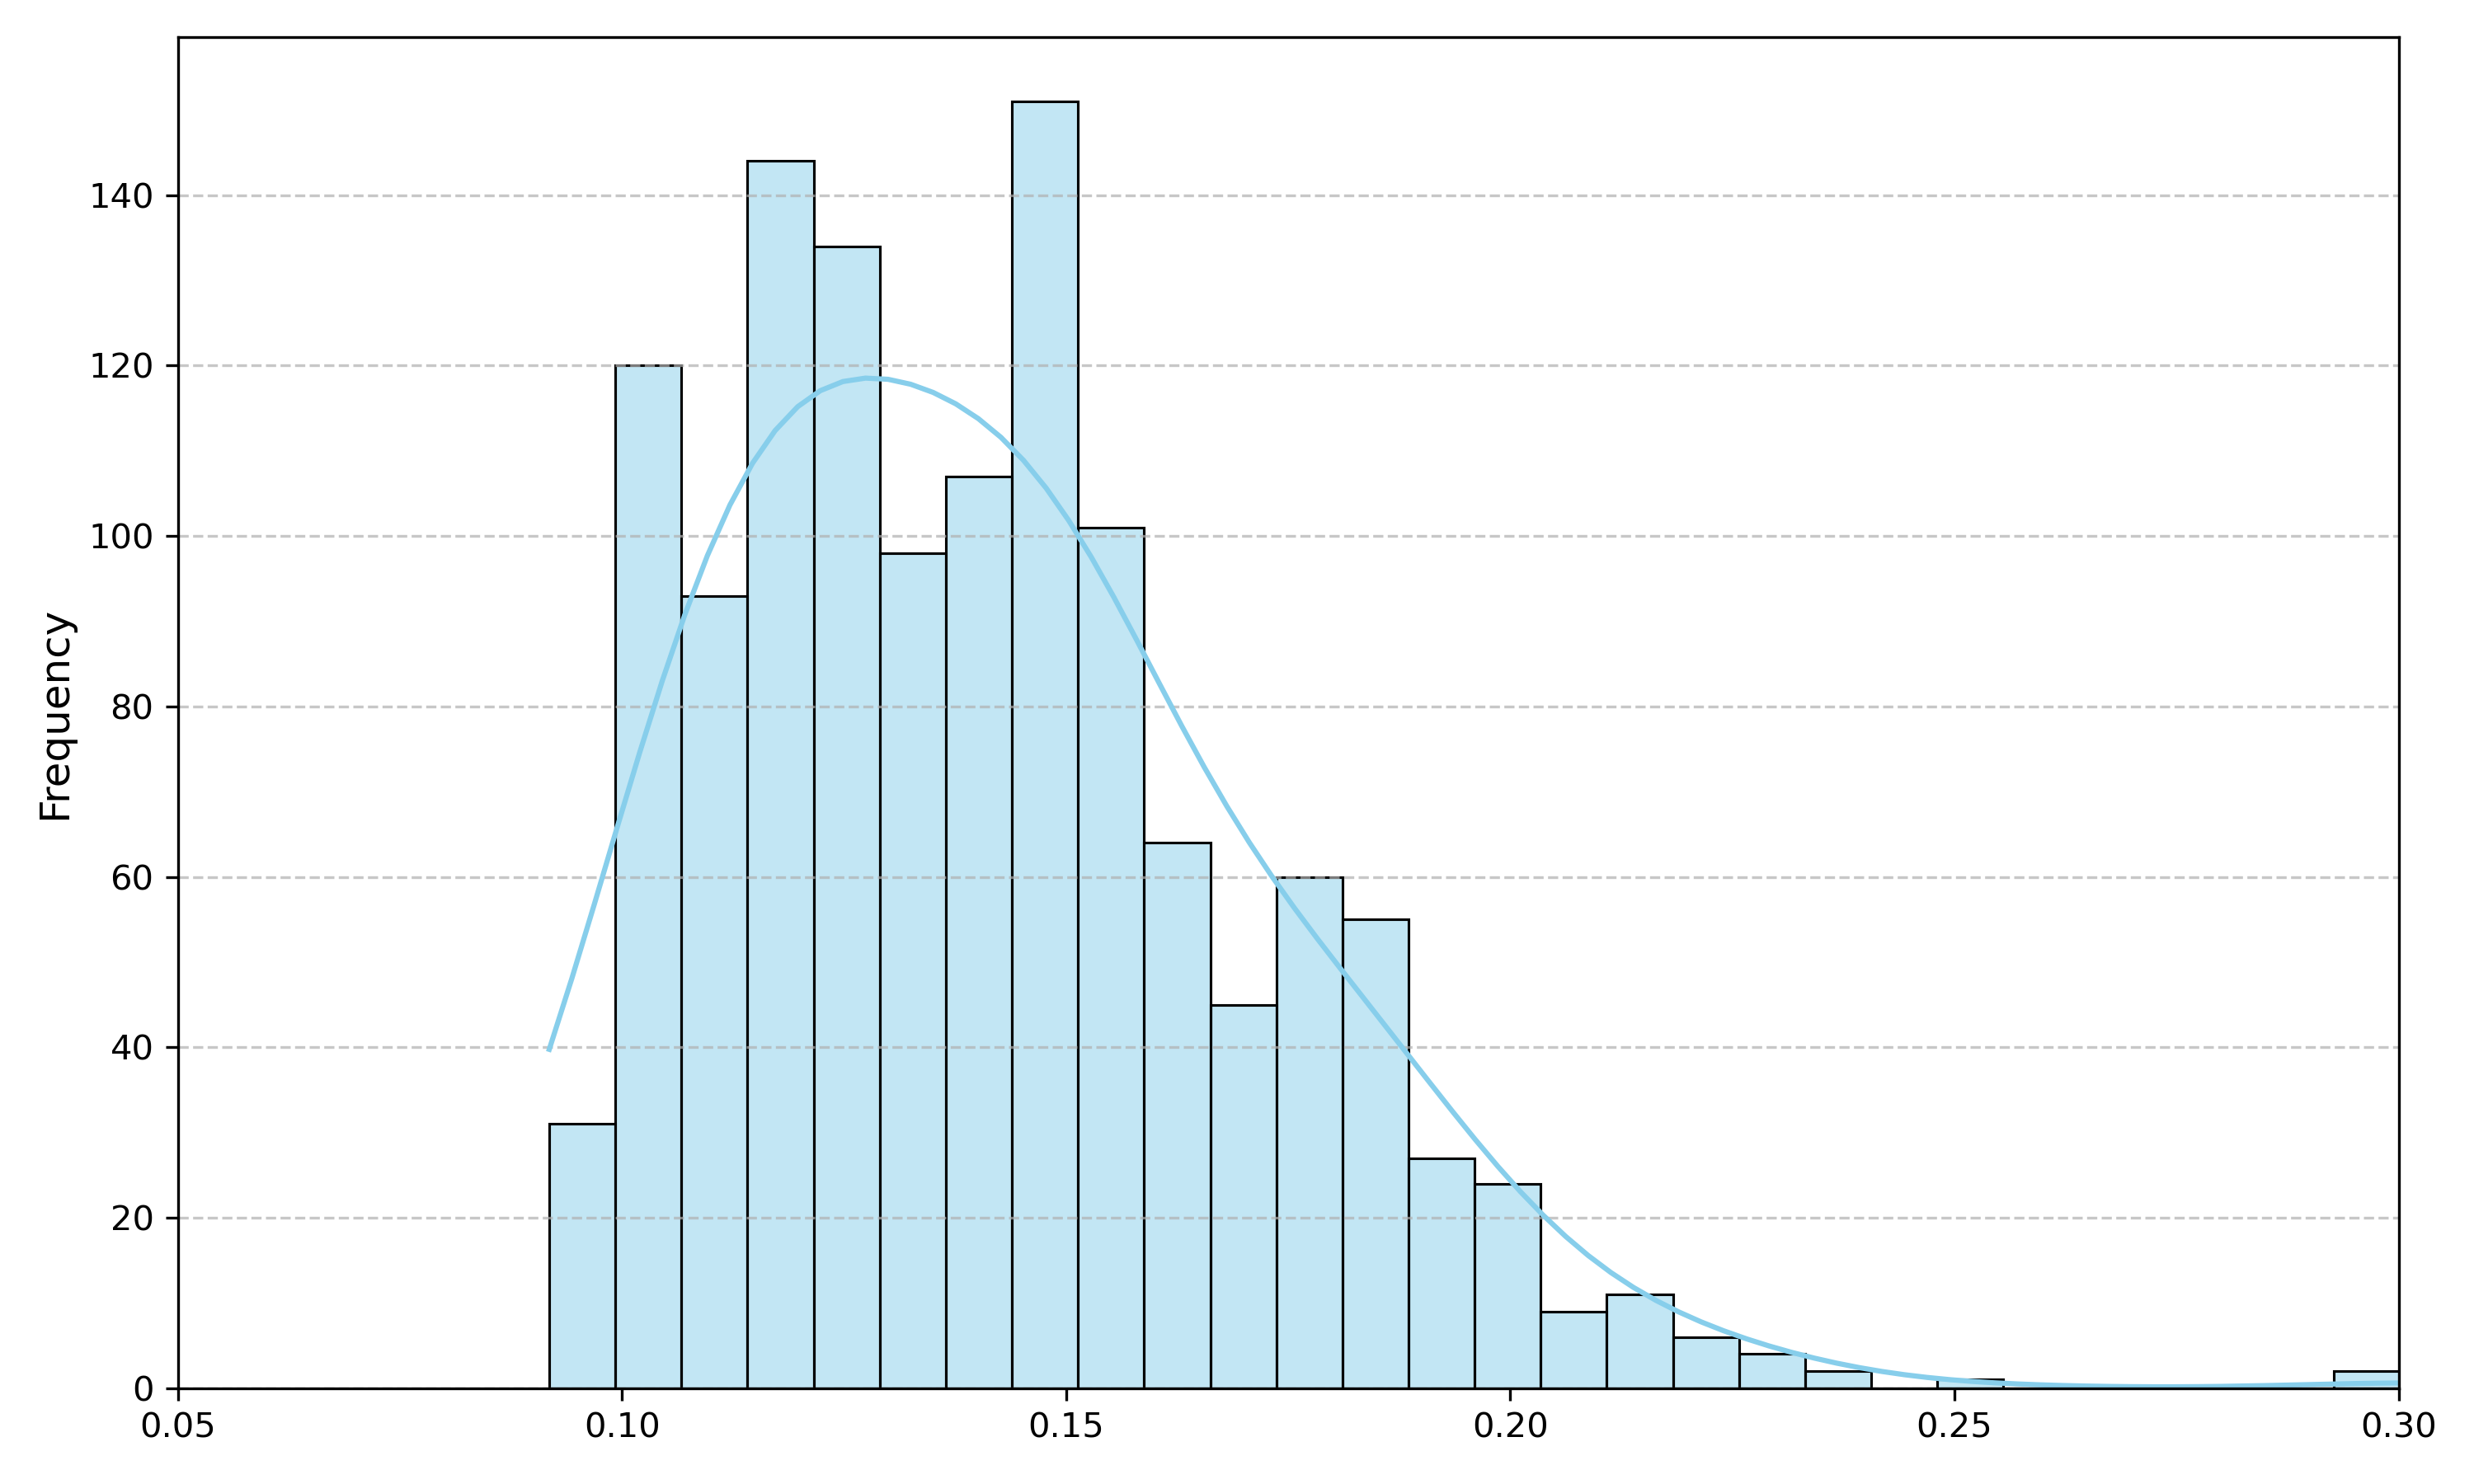
\includegraphics[width=0.8\textwidth,height=0.4\textheight]{new_img/histogram_prosp.png}
            \caption{Distribution of Average Skill Distance (\(\overline{d}_{j_c, t}\))}
            \label{fig:s_dist_hist}
        \end{minipage}
    \end{center}
\end{figure}




\subsection{Empirical Analysis}

Our focus is to develop an understanding of how skill match to vacancies, which we can now measure, affects application 
patterns. Applying is a key step in the internal mobility process and the stage of the search process that can be observed. 
We will look at two aspects of the application process: its directness and intensity. Directness corresponds to whether 
the applicant is applying to positions where they have a higher probability of securing a job, measured using the skill 
distance. Intensity captures how many positions the applicant applies to. Both directedness and intensity improve the 
probability of moving to a new position within the firm. From the firm's perspective, understanding how application 
behavior predictably varies enables them to tweak processes to support employee mobility within the organization. Our 
empirical investigation focuses on three key patterns in application behavior as they relate to the average skill distance 
measure, and we present our findings for each of these patterns in the following sub-sections.


\subsubsection{Average Skill Distance and Application Intensity}

The relationship between an applicant's average skill distance to available vacancies and the positions they choose to 
apply for provides crucial insights into internal mobility patterns. We investigate whether a higher average skill 
distance is associated with applying to closer or farther positions in terms of skill requirements. This analysis 
helps us understand how employees navigate their career paths within the firm when faced with varying degrees of skill 
alignment with available opportunities.

Applicants with a high average skill distance to vacancies face a potentially smaller set of opportunities that closely 
align with their existing skillset. This situation presents a dilemma: do these employees constrain their applications 
to fewer, more closely aligned positions, or do they make more exploratory applications to positions that require 
significant skill development? Conversely, applicants whose skillsets are closer to the available vacancies might 
be less inclined to seek positions that require learning new technologies or skills.

To empirically examine how skill remoteness affects application behavior, we estimate the following model:

\begin{equation}
    d_{j_v, j_c} = \beta_0 + \beta_1 \overline{d}_{j_c, t} + \epsilon
\end{equation}

$d_{j_v, j_c}$ is the standardized skill distance between the current job $j_c$ and the job applied for $j_v$, 
and $\overline{d}_{j_c, t}$ is the standardized average skill distance to vacancies.


\begin{table}[h]
\centering
\caption{Average Skill Distance and Application Intensity} 
\renewcommand{\arraystretch}{1.2}
\begin{tabular}{lcc}
\hline
\textbf{Variable} & \textbf{Coefficient} & \textbf{Std. Error} \\
\hline
Constant & 2.945e-16 & 0.022 \\
$\overline{d}_{j_c, t}$ (std) & 0.6093*** & 0.025 \\
\hline
R-squared & \multicolumn{2}{c}{0.371} \\
\hline
\multicolumn{3}{l}{*** p$<$0.01, ** p$<$0.05, * p$<$0.1} \\
\end{tabular}
\label{tab:skill_remote_app}
\end{table}

The results presented in Table \ref{tab:skill_remote_app} reveal a strong positive association 
between $\overline{d}_{j_c, t}$ and $d_{j_v, j_c}$. Specifically, we find that a one standard deviation 
increase in average skill distance to vacancies is associated with a 0.6093 standard deviation increase 
in the distance to the position applied for. This substantial and statistically significant effect suggests 
that applicants with higher skill remoteness are more likely to apply to positions that are farther away in 
terms of skillset. The application patterns here confirm that when faced with a higher average distance to 
available vacancies, applicants make more exploratory choices. Rather than constraining their applications 
to a narrower set of closely aligned positions, employees appear to broaden their search, potentially seeking 
opportunities that require attaining new skills and capitalize on the firm's knowledge of the applicant's 
performance in the current role which cannot be easily conveyed when applying to a position outside the firm. 
We already know that applying to a more distant position reduce selection chances, but will examine this more closely. 




\subsubsection{Average Skill Distance and Selection Probability}

We've already seen that skill distance is inversely linked to selection probability, and that applicants facing 
higher average skill distance to the set of vacancies tend to apply to more distant positions. Connecting these 
dots, we expect that applicants dealing with higher average skill distances to vacancies are less likely to get 
selected. We examine this here:


\begin{equation}
\text{logit}(P(S_{v,c} = 1)) = \beta_0 + \beta_1 \times \mathbb{I}[\text{above}]_{j_v,j_c}
\end{equation} 

$S_{v,c} = 1$ is a binary variable indicating whether an applicant with current job $j_c$ is selected for the 
job vacancy they applied to $j_v$. The variable $\mathbb{I}[\text{above}]_{j_v,j_c}$ is an indicator function 
that equals 1 if the skill distance between $j_c$ and $j_s$ is above the median, and 0 otherwise. 
Table \ref{tab:selection_prob} presents the results of this logistic regression:

\begin{table}[h]
\centering
\caption{Logistic Regression Results: Impact of Skill Distance on Selection Probability} 
\renewcommand{\arraystretch}{1.2} % Increased spacing
\begin{tabular}{lcc}
\hline
\textbf{Variable} & \textbf{Coefficient} & \textbf{Std. Error} \\
\hline
Constant & -0.0061 & 0.078 \\
Above Median & -0.4083*** & 0.112 \\
\hline
Log-Likelihood & \multicolumn{2}{c}{-895.62} \\
\hline
\multicolumn{3}{l}{\footnotesize{*** p$<$0.01, ** p$<$0.05, * p$<$0.1}} \\
\end{tabular}
\label{tab:selection_prob}
\end{table}

The results align with our expectations. Applicants with above-median skill distance to the vacancies have 
a 33.5\% lower likelihood of being selected into their position. With this we clearly see that the avg. skill distance 
to the vacancies affect the applicant's ability to secure an internal position with the same effort. The natural 
follow up and closely aligned question is of the intensity of the application process which we take up next.


\subsubsection{Average Skill Distance and Application Intensity}

We will now examine whether the application intensity—the number of vacancies an applicant applies to—varies with 
their average skill distance to the vacancy set. We already know that applicants faced with a high $d_{c,t}$ apply 
to more distant positions and are less likely to be selected. Our goal here is to inquire whether they also apply 
to more positions. For this analysis, we slightly modify our approach to constructing application windows. We define 
each window as a sequence of applications where the gap between any two consecutive applications does not exceed 
30 days. This allows for windows that may span longer than 30 days, provided no two consecutive applications 
within the window are more than 30 days apart. We estimate the following regression:

\begin{equation}
    A_{i,t} = \beta_0 + \beta_1 \mathbb{I}[\text{above}]_{i,t} + \epsilon
\end{equation}

Here, $A_{i,t}$ is the number of applications person $i$ submits in time window $t$, 
and $\mathbb{I}[\text{above}]_{i,t}$ indicates if their skill remoteness is above the median.


\begin{table}[h]
\centering
\caption{Average Skill Distance and Application Intensity}
\renewcommand{\arraystretch}{1.2} % Increased spacing
\begin{tabular}{lcc}
\hline
\textbf{Variable} & \textbf{Coefficient} & \textbf{Std. Error} \\
\hline
Constant & 1.8210*** & 0.137 \\
Above Median & 0.5334*** & 0.205 \\
\hline
Observations & \multicolumn{2}{c}{637} \\
R-squared & \multicolumn{2}{c}{0.011} \\
\hline
\multicolumn{3}{l}{\small{*** p$<$0.01, ** p$<$0.05, * p$<$0.1}} \\
\end{tabular}
\label{tab:skill_remote_intensity} 
\end{table}


Table \ref{tab:skill_remote_intensity} shows that applicants with above-median skill remoteness apply to about 1.5 
times more positions on average. Faced with diminished prospects for their skillset within firm opportunities, 
they adopt a more exploratory approach when seeking a new position. Putting all our findings together, we get a 
clearer picture of how skill remoteness to the new vacancies shape internal job applications within the firm. 
Applicants with higher skill distance to the vacancies tend to apply to jobs that are more distant in terms of skills, 
face lower chances of being selected, and submit more applications on average. In other words our skill distance measure 
has allowed to bring out distinct difference in the application patterns to new vacancies. With this understanding, 
the natural follow up question is how we can fine-tune internal mobility processes in the firm? which we take up next.




\subsection{From Mobility Patterns to Practice}

In a technology-focused firm, understanding and supporting internal mobility requires a clear view of how employees' 
current skills align with emerging requirements. Our analysis of job posting content reveals striking patterns in 
how employees navigate opportunities based on their skill-fit - patterns that would be difficult to discern without 
validated measures of skill distance. Employees whose skills closely match emerging opportunities often adopt a 
passive approach despite higher chances of success, while those facing larger skill distances pursue positions 
more actively but with lower success rates.

These empirically-documented patterns point to a clear quantitative framework for workforce development. When employees' 
skills align well with vacancies but application rates are low, the primary barrier appears to be search friction rather 
than skill gaps. As \autocite{invisiblehand} note, managerial initiative in surfacing opportunities can be crucial in 
large firms. Conversely, when employees face high average skill distances to vacancies and apply actively but unsuccessfully, 
the evidence suggests skill development needs rather than search frictions limit mobility. This ability to distinguish 
between friction and skill gap challenges using posting content enables firms to develop targeted interventions.

While our analysis illuminates these distinct patterns, moving from measurement to practice requires careful consideration. 
For employees with low average skill distance who do apply, the data supports proactive opportunity identification. 
However, for those not observed applying, questions remain about how best to surface relevant opportunities. Similarly, 
the application patterns of employees facing larger skill distances provide valuable signals about career directions 
they see as feasible or desirable - opening new possibilities for studying how employees navigate skill requirements 
in modern careers. This suggests rich possibilities for building systematic, evidence-based approaches to workforce 
development by leveraging the skill information in job postings. Rather than relying on generic mobility programs, 
firms can use posting content to quantify where reducing search frictions versus supporting skill development would 
be most valuable, while gaining deeper insight into how employees approach career development in environments of 
evolving skill demands.


